\section{Background}\label{sec:background}

\subsection{Computational Thinking}\label{sec:CTdef}
We start off by explaining the notion of Computational Thinking (CT).

In 2006 Computational Thinking was described by Wing as the extension of every child's analytical ability \cite{Wing2006}. Since then, CT has found its way into primary and secondary curricula around the globe, including the reformed Dutch Curriculum. CT refers to thought processes that are involved when solving complex problems and generalizing and transferring this problem solving process to a wide variety of problems \cite{voogt2015computational}. CT are higher-order-thinking skills \cite{Yadav2017CTteacherEd}.



There is no general consensus on the definition of Computational Thinking \cite{Yadav2015}. \citeA{voogt2015computational} call for a flexible and pragmatic approach and use an operationalization of CT, such as has been done by \citeA{Yadav2015}. \citeA{selby2013computational} sought a narrower definition to facilitate assessment. They tallied occurring terms, descriptions, and meanings for CT in different definitions found in literature. Then, considering the motivation by each individual author for either incorporating or neglecting the term, they came to ordered criteria, which do not necessarily to accommodate all viewpoints. Selby and Woollard \cite{selby2013computational} describe Computational Thinking as a focused approach to problem solving, incorporating thought processes that utilize \emph{abstraction}, \emph{decomposition}, \emph{algorithmic design}, \emph{evaluation}, and \emph{generalizations}. \citeA{BrennanResnick2012} propose three dimensions: Computational concepts (such as variables and loops), practices (such as debugging, abstracting, and being incremental) and perspectives (such as  questioning about the technology world). \citeA{barrStephenson2011CTdef} come to the following set of CT concepts and capabilities: decomposition, abstraction, algorithms, automation, parallelization, simulation and data collection, analysis, and representation.
%
%\begin{itemize}
%\item Algorithmic Thinking: thinking in terms of rules, steps and repetitions (of subtasks).
%\item Decomposition: Breaking a problem into sub-problems (which can be dealt with individually).
%\item Abstraction: simplifying a problem by leaving out (irrelevant) details.
%\item Generalization: finding patterns and re-using solutions (transfer).
%\item Evaluation: Does my solution solve the problem? Analysis: How could process/solution have been improved?
%\item Automation: implementation (through computing tools).
%\end{itemize}


Corradini et al. (\cite{corradini2017conceptions}
compared and analyzed five well-cited definitions (Wing \cite{Wing2006}, CSTA\cite{CSTA2011CT}, Google\cite{Google2017CT}, Brennan and Resnick\cite{BrennanResnick2012}, and Barefoot CAS\cite{CAS2014CT}) to come to common grounds. They grouped common aspects to four categories:
\begin{itemize}
\item \emph{mental processes}: algorithmic thinking, logical thinking, decomposition, abstraction, pattern recognition, generalisation.
\item \emph{methods}: automation, data collection, analysis and representation, parallelization, simulation, evaluation and programming.
\item \emph{practices}: experimenting, iterating, tinkering, testing, debugging, reusing, remixing.
\item \emph{transversal skills}: create, communicate, collaborate, reflect, learn, meta-reflect, and be tolerant for ambiguity.
\end{itemize}

The approaches and attitudes from CAS and CSTA definitions also coincide with the Skills domain in the reformed curriculum. Common aspects are designing, developing, collaborating and communicating. Attitudes, such as CSTA's "mindset to deal with open ended problems, complexity and tolerance for ambiguity" are not specifically mentioned but are pre-requisite to the abilities that are explicably stated (such as "to weigh the options of a digital artefact by means of research and experimentation").



There is a (subtle) difference between CT skills and abilities. An example of an ability is "to formulate problems in such a way that one can use computers and other tools to help solve them" \cite{Barendsen2016}. The CT skill is the performance that a student must do to demonstrate this ability. In the case of the ability to formulate a problem, the relevant CT skills would be applying decomposition and algorithmic thinking.

\subsection{Programming}
In this section we describe the role of programming in CS secondary education, in particular what we know about how to learn and assess it, what students perceive as difficult. In addition we discuss some viewpoints with respect to its relationship with Computational Thinking. Does programming help develop CT skills, or is CT pre-requisite for programming?

Programming is the automation of a solution such that it can be executed by a computer. In this section we describe knowledge, skills, difficulties and approaches to programming.

\subsubsection{Programming knowledge and skills}\label{ProgrammingKnowledgeAndSkills}
Programming requires a combination of conceptual knowledge and skills. In addition to the syntax of a particular programming language, it requires knowledge about concepts (just to name a few: loops, conditionals, and mathematical and logical operators) and the notion of the machine (how the computer interprets and executes the commands, for example, that the code in a function definition is not executed if the function itself is not called). Moreover, as code grows in magnitude or complexity, aspects such as decomposition and abstraction come into place to keep the code manageable and robust. Coding also involves practices such as iterating, tinkering, testing and debugging. And furthermore, attitudes and transversal skills, such as (meta-) reflection, communication and collaboration, being tolerant for ambiguity, and last but not least, being persistent when dealing with open-ended or complex problems play a role. All-in-all, programming requires a plethora of knowledge and skills.


Several studies report an evident link between programming and CT. In his analysis Hu \cite{hu2011computational} state that developing computational thinking skills would make students better prepared and more successful in learning programming.\todo{uit def 1 can de 4 artikelem ook menselijke agent}\todo{Also lots of unplugged + cite} \citeA{Yadav2017CTteacherEd} expresses that creating computational artifacts increases creative expression and thus problem solving skills. \citeA{BrennanResnick2012} use programming to develop computational thinking. And in their review study, \citeA{LyeKoh2014} analyse different ways of exposing students to computational thinking through programming. However, IT devices are not absolutely needed to develop CT competencies in students\cite{corradini2017conceptions}. In their analysis of the most cited CT definitions, \cite{corradini2017conceptions} describe CT as the formulation of a solution to a problem such that a processing agent can carry it out. They mention explicitly that this processing agent can be either human or a machine. This idea is reinforced by the vast number of 'unplugged' lessons being developed which teach CS and programming without the use of a computer, but rather through kinesthetic activities and engaging games, puzzles and magic tricks (\cite{curzon2009CT}, \cite{CSUnplugged}, \cite{CSFieldGuide}). \citeA{davies2008effects} focus on teaching CT skills prior to a programming language, and conclude that such an approach enhances programming skills.


In his article, \citeA{denning2017remaining} differentiates between traditional CT (prior to the 2006 Wing 'movement') and new CT. Where in the traditional CT, programming ability is described to produce CT, and in the new, CT is a conceptual framework that enables programming. In the new CT, programs are loosely coupled with algorithms and translation it into a program is optional. The solution of the problem must be expressed precisely and unambiguously in a way that a processing agent can carry it out, but for all that matters, that processing agent can be either a human or a machine\cite{corradini2017conceptions}.

What is important to take away from this discussion, is that there is a fundamental difference between CT and programming. CT encompasses the design of an algorithm. A flowchart could be used to articulate and visualize an algorithm. This does not require interaction with a processing agent (i.e. a machine). Programming pertains to implementation, knowledge about using concepts and constructs of a programming language and the skills to translate the algorithm into code and creating a digital artefact.

So, in order to assess both CT and programming knowledge and skills requires evidence elicited from several products or activities.

%In a survey of program understanding, von Mayrhauser and Vans
%(1994) summarise studies (in particular Guindon, 1990) noting that experts:
%have efficiently organised and specialised knowledge schemas; organise their
%knowledge according to functional characteristics such as the nature of the
%underlying algorithm (rather than superficial details such as language syntax);
%use both general problem solving strategies (such as divide-and-conquer) and
%specialised strategies; use specialised schemas and a top-down, breadth-first
%approach to efficiently decompose and understand programs; and are flexible in their approach to program comprehension and their willingness to abandon
%questionable hypotheses.[Robins, Rountree, Rountre (2003).  ]
\subsubsection{Programming difficulties}


Sources of programming difficulties (or 'misconceptions') which novice programmers encounter have been extensively researched and documented. Misconceptions can keep students from producing correct programs (efficiently). In their meta-analysis, \citeA{Sheard2009} investigated 164 relevant full-refereed papers about programming education. \citeauthor{robins2003learning} gives a general account of misconceptions \cite{robins2003learning}. Others focus on specific concepts such as variables \cite{Kuittinen2004}, loops \cite{Dancik2003}, functions (and parameters)\cite{sorva2012misconceptions}, boolean conditions and control structures \cite{Almstrum1999, Herman2010}. \citeA{spohrer1986novice} analyze difficulties related to \emph{plan composition} problems, and argue that these have even more impact on programming errors than construct-based misconceptions.


%Researchers have catalogued a vast number of misconceptions pertaining to programming\todo{(see [3, 27] for reviews of these studies)}. Misconceptions can keep students from producing correct programs (efficiently). In their research, \cite{sorva2012misconceptions} investigate common misconception-related mistakes made by students and categorize these according to basic concepts, functions and object-oriented programming. The most common misconceptions they found which are relevant for secondary education are:
%\begin{itemize}
%\item Inverted assignment: the student erroneously assigns the value of the left-hand variable to the right-hand side variable.
%\item Selection: in an if-then-else statement, the then-branch is always executed
%\item Confusing the assignment ('=') and comparison ('==') operators.
%\item Not understanding the role of variables in the condition of a while loop.
%\item Executing a function instead of defining it.
%\item Parameters
%\item Return values
%\end{itemize}


% misconception
%researchers have catalogued a vast number of misconceptions
%about computer behavior and basic programming constructs
%(see [3, 27] for reviews of these studies).
%M. Clancy. Misconceptions and Attitudes that Interfere
%with Learning to Program. In S. Fincher and M. Petre,
%editors, Computer Science Education Research, pages
%85–100. Routledge, 2004.
%
%J. Sorva. Visual Program Simulation in Introductory
%Programming Education. Doctoral dissertation,
%Department of Computer Science and Engineering,
%Aalto University, 2012.

\todo{and misconceptions}
\todo{sorva}

\subsubsection{Programming Strategies and Plans}\label{sec:plans}




One of the skills needed for programming is dealing with complexity\todo{is dit zo, of kun je beter open-ended of ambiguousu gebruken}. As programs increase in magnitude, aspects such as decomposition, modularisation, and generalisation become important. The enable the programmer to interpret and oversee the program as a whole (and thus on a relational level). \citeA{deRaadt2009teachingPlans} describe a set of elementary plans (i.e. programming strategies) that can be combined in different ways to create solutions. Examples of elementary plans are Initialization plan (variables), Average plan, Triangular Swap plan, Guarded Division plan, Counter-Controlled Loop plan, Sum and Count plans, Bubble Sort algorithm. They explain that the identification, selection and application of plans can be seen as a representation for strategy (similarly described by Soloway (1985), also known as applying patterns (Wallingford, 1996)) and should be taught and assessed explicitly. The new Dutch curriculum \cite{Barendsen2016}\todo{eingenlijk de handreiking} refers to some of these plans, such as the Maximum, Sum and Sort plans.

Plans or strategies can be expressed both simply, at a subalgorithmic level, and at a higher level\cite{deRaadt2006}. A higher birds-view level in which one reasons about the purpose of a program holistically, combining relevant aspects and analysing a program as an entity, corresponds to multistructural or relational level in terms of the SOLO taxonomy\cite{Smetsers2017}. Meanwhile, describing a program at a subalgorithmic level in corresponds to unistructural level in terms of the SOLO taxonomy. Thus the distinction between these levels coincide with the SOLO categories, as described by \citeA{lister2010naturally}, \citeA{Meerbaum2013} and Meerbaum-Salant et. al. (2010).

A number of attempts have been made to decompose these strategies (Muller, Haberman, and Ginat, 2007; Porter and Calder, 2003; Wallingford, 2007)\todo{ Erik: uitsplitsen en toelichten wat ieder gedaan heeft zodat je dit als lezer niet zelf hoeft op te zoeken} into smaller units and distinguish pre-requisite knowledge. Recognizing and applying plans as higher-level algorithms relates to multi-structural and relational levels in the SOLO taxonomy. They enable reasoning in terms of plans and goals, rather than low-level lines of code. Soloway (p. 856) and de Raadt identify the following methods of integrating plans (bottom-up):
\begin{itemize}
\item Abutment: plans following each other in sequence. For example, initializing a variable and printing it’s value:
\begin{PYTHON}
x=12
print("The value of x is: ", + str(x) )
\end{PYTHON}


\item Nesting: one plan as a whole is submerged in another. For example, printing the value of a variable during intermediate iterations of a counting plan:
\begin{PYTHON}
counter=0
while not done():
    counter+=1
    print("The number of items is: " + str(counter))
\end{PYTHON}

\item Merging: interleaving (at least) two plans. For example,the averaging problem merges input, summing and counting plans.
\end{itemize}

\citeauthor{deRaadt2009teachingPlans}'s research is not directly applicable to secondary education. Underlying concepts at a basic unistructural level which may assumed to be trivial (at CS1 level), may not be so trivial at all in secondary education. For example, the 'average plan', explicitly states the need to understand the division operator, but doesn't say anything about pre-requisite knowledge about the assignment of variables. There are also other concepts which are (explicitly or implicitly) stated in reformed CS curricula but not included in the plans. These are: procedures, functions, parameters, and a Boolean-Flag loop plan as a specific form of a primed sentinel controlled loop plan. That it is essential to regard these concepts, even, or especially at a unistructural level becomes apparent from the long lists of related misconceptions that researchers and educators have established. Misconceptions about these concepts has been researched and documented, for example by \citeauthor{sorva2012misconceptions} and \url{PD4CS.org}.



\subsection{Algorithms, Algorithmic Thinking, and Problem Solving}
Computational problem-solving, logical and algorithmic thinking have been identified as aspects of CT [Grover2017Assessmnet]. In this section we describe its relationship with algorithms, in light of CS secondary education.


\citeA{Wing2006} describes CT as a linking pin in CS: "solving problems, designing systems, and understanding human behavior, by drawing on the concepts fundamental to computer science". ISTE and CSTA define CT as "a problem-solving process"\cite{CSTA2011CT} and characterize it as "automating solutions through algorithmic thinking". The reformed curriculum refers to computational thinking and problem solving in the \emph{Using informatics as a perspective} sub-domain: "analytical skills to formulate problems in such a way that one can use computers and other tools to help solve them, as well as problem solving skills,
such as finding solutions in terms of algorithms and data"\cite{Barendsen2016}. This coincides with the ISTE-CSTA definition.




Algorithms are a fundamental CS concept. \citeA{gal2002efficiency}'s review of international university and high school curricula, show that the concepts of algorithms and algorithm efficiency are central to the study of CS. Algorithms are tools for developing and expressing solutions to computational problems (\cite{GroverPea2013}).


Algorithmic thinking pertains to abilities needed to construct and understand algorithms that solve given problems. \citeA{futschek2006algorithmicThinking} distinguishes the following abilities:
\begin{itemize}
\item analyze given problems
\item specify a problem precisely
\item construct a correct algorithm to a given problem using basic actions
\item think about all possible special and normal cases of a problem
\item improve the efficiency of an algorithm
\end{itemize}
Based on the CT definitions from \cite{CAS2014CT}, \cite{Google2017CT}, \cite{BrennanResnick2012} and \cite{CSTA2011CT}, Algorithmic thinking is the process of designing a sequence of ordered steps (thus an algorithm) to solve a problem, achieve a goal or perform a task\cite{corradini2017conceptions}. Algorithmic thinking can be viewed as aspects of Computational Thinking (CT) as it involves abstraction and decomposition of open-ended problems, the construction of a solution through algorithmic thinking, generalization and the evaluation of its result \cite{Wing2006}.



Computer science learners often experience difficulties during problem analysis, planning and design of solutions \cite{Hazzan2011}. \citeA{kirschner2006minimal} argue that learning a complex task like programming, not only requires conceptual knowledge, but also \emph{explicit procedural guidance}. It is essential to understand which steps must be taken in order to solve a problem, as well as how to recognize an acceptable solution.


\citeA{McCracken2001} describe five iterative steps to problem solving (PS). The steps also coincide with the steps that Polya describe in his book "\emph{How to solve it}" on problem solving \cite{polya2004solve}. They also encompass each of the CT skills as described by \citeA{selby2013computational} after comparing and contrasting CT definitions in an extensive literature review.  Table \ref{table:problemSolvingCT} shows how these three coincide. The step of integrating sub-solutions (via abutment, merging and nesting) corresponds with algorithmic thinking, as it involves creating an algorithm that controls the sequence of events. An important aspect of the reverse step, generating sub-problems, is recognizing plans, existing methods or strategies. Recognizing plans at an abstract level helps decompose the problem and simplifies reasoning about its solution (\cite{Smetsers2017}). What remains is to fine-tune the plan to the specific situation and then integrate it with the remaining sub-solutions. To be successful in developing novel algorithms that solve problems correctly and successfully, calls for a coherent set of skills and knowledge.



\begin{table*}
  \centering
\begin{tabular}{|l|l|l|}
  \hline
  % after \\: \hline or \cline{col1-col2} \cline{col3-col4} ...
  \textbf{\citeauthor{McCracken2001}'s PS} & \textbf{\citeauthor{polya2004solve}'s PS} & \textbf{\cite{selby2013computational}'s CT} \\
  \hline


    Abstract the problem from its description & Understand the problem & Abstraction, Generalization \\ \hline

    Generate sub-problems & Make a plan & Decomposition \\ \hline

    Transform sub-problems into sub-solutions & Carry out the plan & Algorithmic thinking \\ \hline

    Re-compose the sub-solutions into a working program & Carry out the plan & Algorithmic thinking \\ \hline

    Evaluate and iterate & Look back on your work & Evaluation \\ \hline

  \hline
\end{tabular}
\caption{Problem solving and CT}\label{table:problemSolvingCT}
\end{table*}





Plans (as described in section \ref{sec:plans}) enable reasoning on a higher level of abstraction. Decomposing complex problems (or solutions), recognizing relevant plans and incorporating them into a solution facilitates reasoning about the purpose, correctness, and efficiency of code.  The use of plans thus assists students to deal with open-ended problems.

In 1974, Donald Knuth said that articulating a solution as an algorithm and implementing (and testing) the concept on a computer leads to a deep understanding of concepts of all kinds in many fields. CT thought processes are involved in formulating problems so their solutions can be represented as computational steps and algorithms\cite{aho2012computation}. On the one hand, algorithmic thinking (as part of CT) and problem-solving skills are essential for programming, and thus developing algorithms(\cite{McCracken2001}). On the other, fundamental knowledge of the concepts of algorithms are needed, i.e., how algorithms work, which common algorithms and plans exist, and knowledge about strategies for composing (or combining) algorithmic components\cite{deRaadt2008}. In his article, \citeA{denning2017remaining} explains that learning certain concepts produces programming ability, rather than the other way around.





\todo{How to develop skills and reinforce knowledge related to algorithms… either through concepts or programming. <SEE VERHAAL VAN DENNING, 2017>}





\subsection{Assessment and criteria(THEORY)}
This section will discuss what we know about assessments, such as taxonomies and pathways.


Assessments are used for several purposes. \citeA{mcmillan2007formative} distinguishes between two types of assessments, summative and formative. Summative assessment refers to the use of assessment-based evidence to help us arrive at go/no-go decisions based on the success of a completed course or instructional program (\cite{popham2009assessment}). On the other hand, assessment for learning is formative. Formative assessment is used by both students and teachers to adjust ongoing instructional and learning activities in order to improve the manner in which learning is taking place. Summative assessment can also be treated formatively, for example to determine the effectiveness of instruction.




A substantial amount of research has been done into the role of assessment in education. In his study Frederiksen (\cite{frederiksen1984}) describe assessment as a motivator for learning. Alderson and Wall (1993) and Prodromou (1996) elaborate by stating that what is assessed strongly influences what is learned. Biggs (\cite{biggs1996}) prescribes that instruction, learning, and assessment must be well-aligned. This alignment exists in most traditional knowledge-based tests, yet constructive alignment for competency-based instruction is not self-evident (\cite{baartman2006wheel}). With the emphasis of Computational Thinking and problem solving in reformed CS curricula, learning and instruction is increasingly competency-based. Assessment of competencies is complex, mainly because it comprises a multi-facetted blend of knowledge, skills and attitudes (\cite{merrienboer2002competenties}).


As discussed in section \ref{ProgrammingKnowledgeAndSkills}, though they complement each other, CT and programming are fundamentally different. CT is a skill and this tacit knowledge should be assessed directly\cite{denning2017remaining}. Assessment should thus elicit behaviors which indicate that a student can master the competency. As Denning formulates it: "\emph{given that so much education is formulated around students acquiring knowledge, looking carefully at skill development in computational thinking is a new and challenging idea}."\cite{denning2017remaining}\todo{Erik: alignment = validity +?}




\subsubsection*{Assessment Criteria}\label{sec:qualityCriteria}
Effective assessments call for qualitative assessment techniques. Extensive research has been done into the characteristics of qualitative assessments. In this section we discuss the characteristics for knowledge-based (pertaining to CS concepts) and (CS and CT) competency-based assessments.

\todo{dan moet je hier ook iets over knowledge based zeggen.... die gaan sowieso op, competenty komt erbij}

Instruction and learning based on competencies, such as CT, call for assessment methods to adequately determine competency acquisition. Because of the multi-facetted nature of competency assessment, one single assessment method seems not to be sufficient. \citeA{baartman2006wheel} proposes a 'wheel of competency assessment' framework of quality criteria for competency-based assessments, based on a combination of different assessment methods. The diagram below illustrates the different aspects.


%
%\begin{figure*}
%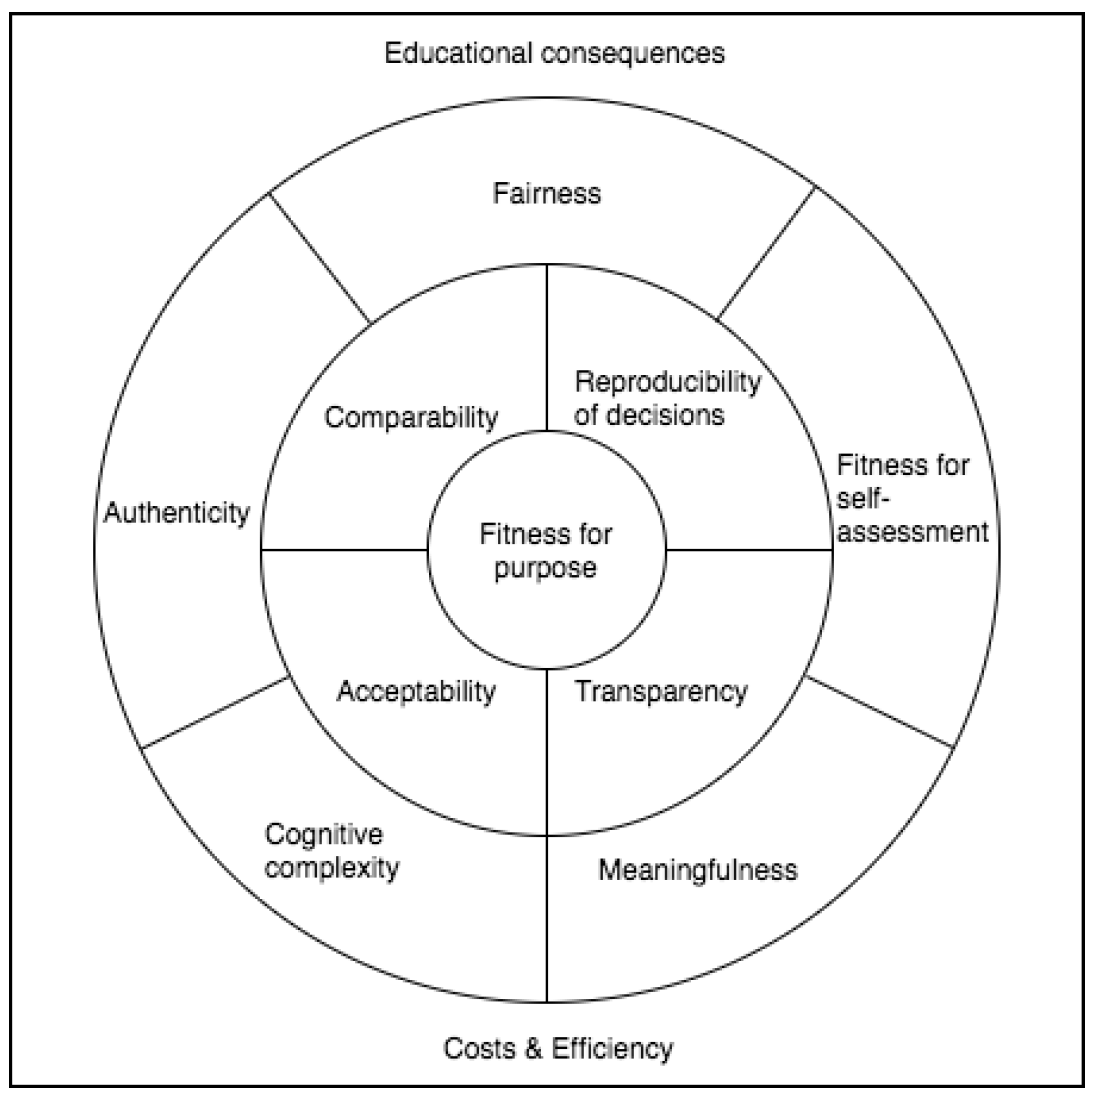
\includegraphics[scale=0.6]{figures/AdaptedQualityCriteriaCatete.png}
%\caption{The Wheel of Competency Assessment (2017Catete)}\label{fig:AdaptedQualityCriteriaCatete}
%\end{figure*}

\begin{center}
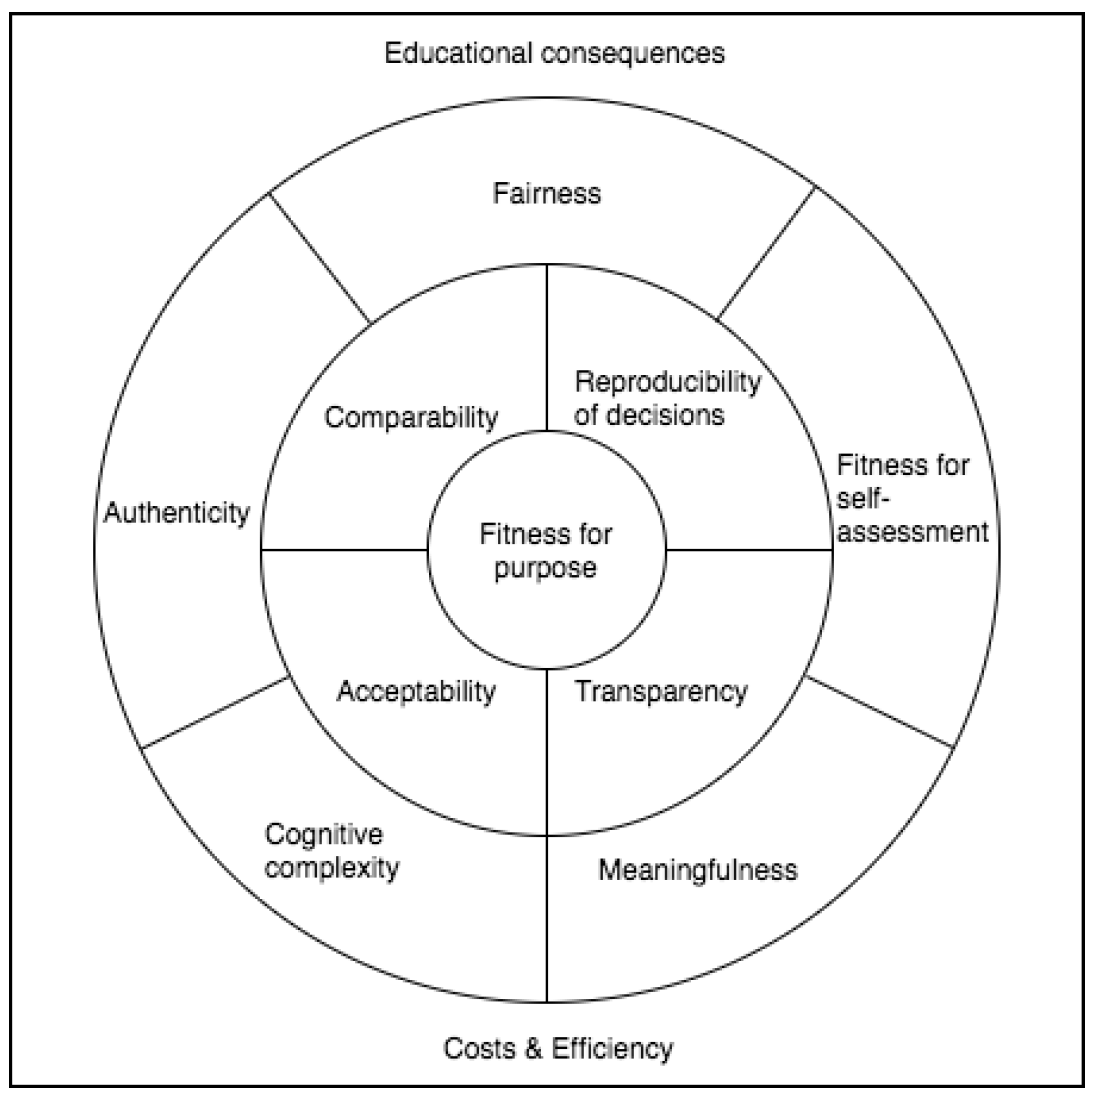
\includegraphics[scale=0.6]{figures/AdaptedQualityCriteriaCatete.png}
The Wheel of Competency Assessment \cite{baartman2006wheel}\label{fig:AssQualityCriteria}
\end{center}


It constitutes the following quality criteria:

\begin{itemize}
\item \emph{Fitness for purpose}: There is alignment between assessment, learning process and instruction.

\item \emph{Comparability}: Scoring occurs in a consistent manner using the same criteria for all learners.

\item \emph{Acceptability}: The assessment is accepted (according to attitude and views) by the professional community.

\item \emph{Transparency}: The assessment is clear and understandable to all participants. \note{A possible indication is to check whether learners can judge themselves and other learners as accurately as trained assessors.}

\item \emph{Reproducibility of decisions}: Accurate evaluation of the evidence independent of the assessor or specific assessment situation. \note{It is not necessary for decisions to be objective to be reproducible.}

\item \emph{Authenticity}: The assessment evaluates competencies needed in the future workplace.

\item \emph{Fairness}: The assessment tests only relevant knowledge, skills and attitudes. It is unbiased towards a certain group of learners (i.e., no unfamiliar and/or unrelated cultural aspects).

\item \emph{Cognitive Complexity}: Assessment tasks reflect the presence of higher cognitive skills and elicit the thinking process used by experts to solve complex problems.

\item \emph{Meaningfulness}: The assessment is significant to both teachers and learners. \note{A possible way to increase meaningfulness is to include learners in the development of the assessment process.}

\item \emph{Fitness for Self-Assessment}: The assessment criteria are clear and indicate weaknesses.\note{ assists in self-regulated learning by making clear what the criterion are, by showing weaknesses and by stimulating reflection on the learning process.}

\item \emph{Educational Consequences}: The intended and unintended effects of the assessment cause teachers and learners to view the goals of education and adjust their learning activities in a positive manner.

\item \emph{Costs \& Efficiencies}: The time and resources needed to develop and carry out the assessment are justified by the positive effects, such as improvements in learning and teaching.

\end{itemize}



in addition the following other success criteria have been mentioned in CS assessment literature:
\begin{itemize}
\item availability and ease of access \cite{Yadav2015}
\item fun and engaging \todo{cite}
\item \ldots \todo{toevoegen, incl cite}
\end{itemize}
\note{2017Catete geeft een mooi overzicht van de aspecten van de wheel, pg 100}

% KOMEN TOCH GEWOON OVEREEN MET REPRODUCIBILITY AND FAIRNESS?
%The framework has been extended by  \citeauthor{catete2017framework} with classical psychometric quality criteria to construct quality-assured programming rubrics for AP CS Principles:
%\begin{itemize}
%\item validity: the ability for the assessment to measure what it is supposed to measure.
%\item reliability: the ability for a student’s work to repeatedly score the same marks on the same rubric.
%
%\end{itemize}


\subsubsection*{Evaluation models}\label{sec:evaluationModels}
\noindent \textbf{Rubrics}\todo{ook iets vertellen over andere evaluation models.. toets matrijs, voorbeeld uitwerking?, etc?}


Rubrics are one of the most common assessment tools used to evaluate student projects. Rubrics use descriptive measures to separate levels of performance on a given task. While grading a particular task, each level is assigned a value. Rubrics are important to use because each student project is rated individually against the same criteria, thus increasing comparability. Rubrics can increase transparency (what is being assessed and how) and reproducibility (accurate evaluation independent of the assessor). Rubrics help clarify expectations for students and teachers, while also speeding up grading\cite{catete2017framework}.



Rubrics can be either holistic or analytical. Table \ref{table:RubricsHolisticAnalytical} summarizes the differences.

\begin{table*}
  \centering
\begin{tabular}{|l|l|l|l|}
  \hline
  % after \\: \hline or \cline{col1-col2} \cline{col3-col4} ...
  \textbf{Type} & \textbf{Evaluation description} & \textbf{Pros} & \textbf{Cons} \\
  \hline
  Holistic & Project rated as a whole & Quick and efficient & Lack specific descriptive measures, no specific feedback on how student can improve, irreproducibility: teachers may disagree about the score \cite{catete2017framework} \\
  Analytical & Each descriptive measure is rated individually & Give specific feedback on how student can improve, can be used for self-assessment & Take longer to design \\
  \hline
\end{tabular}
\caption{Comparison between holistic and analytical rubrics}\label{table:RubricsHolisticAnalytical}
\end{table*}

\citeA{catete2017framework} distinguishes between two types of descriptive measures in rubrics, the learning-based rubric which is learning-goal oriented, and performance-based rubrics which evaluate the end product.

While revisiting the \citeauthor{McCracken2001} working group research, \citeA{mccartney2013assessmentsProgramming} assessed programs using the same two sets of criteria: General Evaluation (largely objective and
based on black-box testing) and Degree-of-closeness (a subjective measure based on the code structure, function and how close to working the program was).


\subsubsection{Taxonomies for the assessment of programming}\label{sec:taxProgramming}

Taxonomies provide a language for describing learning outcomes and performance in assessments. These can be divided into domains (such as cognitive, affective, and psychomotor) or categories based on complexity of the task. Two widely used taxonomies for assessment of learning are the (revised) Bloom taxonomy (Anderson et al., 2001) and the SOLO taxonomy. Both have been used in CS education research, for example, the revised Bloom by \citeA{Whalley2006} and SOLO by Lister et al. (\cite{lister2006not}\cite{lister2010naturally}).

\noindent \textbf{Revised Bloom Taxonomy}\newline
Bloom's taxonomy was designed to aid systematic assessment. It distinguishes between different types of learning objectives (from simple understanding to complex creating) and across multiple domains of learning (from concrete factual, conceptual, procedural, to abstract meta-cognitive). Figure \ref{fig:BloomsRevised} depicts the hierarchy of the types of learning objectives.


%\begin{figure*}
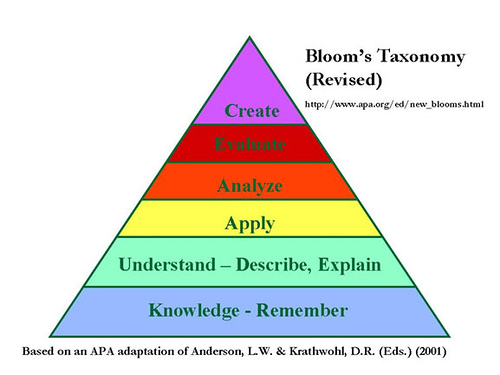
\includegraphics[scale=0.6]{figures/bloomsrevised.jpg}
Revised Bloom's Taxonomy (\cite{krathwohl2002revision})
%\caption{Revised Bloom's Taxonomy (2002Krathwohl)}\label{fig:BloomsRevised}
%\end{figure*}


Drawbacks of Bloom's taxonomy in CS have been reported. \citeA{thompson2008bloom} conclude that experts have difficulties applying Bloom's taxonomy consistently in introductory programming courses. \citeA{Meerbaum2013} similarly report issues with classification, and relate them specifically to the nature of the tasks. \citeA{lister2003} describe that, depending on the magnitude, the act of writing code can belong to either understanding, applying or creating, and code-tracing can belong to remembering, understanding, or  analyzing. \citeA{Whalley2006} express that Bloom's taxonomy is helpful for generating example tasks, but had difficulty placing them within the revised taxonomy. As a result, all comprehension (reading) questions were categorized into one and the same level, namely understanding. Classification becomes meaningless if every task, irrespective of its complexity, falls into the same category.


\noindent \textbf{SOLO Taxonomy}\newline
\citeA{biggs1996} proposes the Structure of the Observed Learning Outcome (SOLO) taxonomy, which classifies learning outcomes in terms of their complexity. The SOLO taxonomy differentiates between a local and a holistic perspective. Understanding can reside along the following scale:
\begin{itemize}
\item \emph{prestructural}: incompetent,
\item \emph{unistructural}: able to identify one relevant aspect,
\item \emph{multistructural}: able to combine several relevant but independent aspects,
\item \emph{relational}: able to analyse or apply that what is integrated into a structure, and
\item \emph{extended abstract}: being able to generalize to a new domain.
\end{itemize}
 As such, the scale can be used to discriminate between being able to read code line-by-line (but not understanding its purposeful intent) from fully understanding and summarizing the goal of a piece of code as an entity. Due to this perspective, SOLO's framework can be used for holistic marking \cite{Fuller2007}. Which type of cognitive processing is involved, such as recalling items or drawing conclusions, are not part of the framework.\todo{Erik: dit herfomuleren... solo rich }


Given the difficulties in categorizing programming activities within the existing taxonomies, several attempts have been made to propose new taxonomies which may be more appropriate for CS education. \citeA{Fuller2007} suggest to separate Bloom’s levels into two dimensions, producing (writing/composition) and interpreting (reading/comprehension). \citeA{lister2003} attempt to differentiate in terms of magnitude of the code (i.e. number of lines of code). Lister et al. \cite{lister2010naturally} propose a refinement of the SOLO taxonomy to account for both the practical and conceptual learning goals in CS. For example, they propose an extension of the taxonomy for code-writing questions by considering a degree of 'partial correctness' for each level on the scale.

\todo{Erik: oorspronkelijk SOLO is door meerbaum vertaald naar lokaal/globaal code beschrijven, deze eigen draai die ze er aan gegeven hebben is essentieel voor informatica. UITBREIDEN en toelichten hoe belangrijk dit is geweest}
\citeA{Meerbaum2013} propose a novel hierarchical taxonomy scale describing how a student’s performance grows in complexity. It’s aim is to pinpoint (the development of) programming skills and spans both problem solving (such as plan composition) and (construct-based) language aspects. It is based on a combination of the Revised Bloom and SOLO taxonomies.  It grasps the best of both worlds into a format specifically applicable to programming: the cognitive categories (understanding, creating) are captured by Bloom, whilst the capability to fully understand or create a program on a holistic perspective (which by definition tackles the magnitude of code issue) is captured by SOLO. The result is a nine-level taxonomy with the highest level being relational creating, and the lowest level being unistructural understanding (on one axis: understanding, applying, creating; on the other: unistructural, multistructural, relational):


%Meerbaum-Salant et al. (2013) propose a hierarchical taxonomy
%scale based on a combination of the revised Bloom and Solo taxonomies
%\cite{Meerbaum2013}. Three super-categories - unistructural, multistructural,
%and relational (derived from the Solo taxonomy) were chosen, each containing
%three sub-categories - understanding, applying, and creating (derived from
%the revised Bloom's taxonomy:

\begin{description}[leftmargin=1em]
\item[Understanding:] The ability to summarize, explain, exemplify,
    classify, and compare CS concepts, including programming constructs.
\item[Applying:] The ability to execute programs or algorithms, to track
    them, and to recognize their goals.
\item[Creating:] The ability to plan and produce programs or algorithms
    (constructing, analysing, evaluating and formulating).
\item[Unistructural:] The ability to create very small scripts doing one
    thing, or adding an instruction with a local effect to an existing
    script.
\item[Multistructural:] The ability to track a program and grasp various
    parts but not the entity they form as a whole.
\item[Relational:] The ability to fully understand a complex concept (such
    as concurrency) and to coherently explain its various facets.
\end{description}

\citeA{Meerbaum2013} conclude that their novel taxonomy enabled them to overcome some of the obstacles with respect to the Bloom or SOLO taxonomies. They acknowledge that more research is needed. One aspect is to consider a continuum between cognitive categories, another is whether the task or concepts involved may overrule the effect of SOLO complexity.



Though the proposed taxonomies have their differences, they all consider two important coding aspects: reading (comprehension) versus writing (composition), and the complexity of the problem.


\todo{Classifying tasks is not straightforward: (\cite{Fuller2007}, \cite{LuxtonReilly2018},  Hu, and Robbins, 2008)}


\subsubsection{Research about assessing programming}\label{sec:researchAssProgramming}
In this section we discus a review of the research about programming assessments.

Assessment tasks should adequately indicate a students’ programming comprehension and clearly discriminate between achieved performance levels.
%ASSESSING UNISTRUCTRURAL CONCEPTS IS A CHALLENGE
A substantial body of work has previously explored the assessments used in novice programming courses in tertiary education. In prior work, researchers claimed that the subject itself was difficult. \citeA{McCracken2001} discuss how students fail to complete tasks, and \citeA{robins2003learning} associate it with high dropout rates in introductory programming courses. The 2001 ITiCSE report by the McCracken Group (\cite{McCracken2001}), a keystone in assessment literature (\cite{Giordano2015}) on CS concepts, describes the difficulties pertaining to the development and validation of assessment activities. They raise concerns about task selection and the difficulties of standardizing assessments for multiple institutes.  \citeA{lister2004multi} gave students two types of multiple choice questions. The first to predict the outcome of a short piece of code and the second finish near-complete code. Students were weak at both tasks, especially the latter. Using that work as a starting point, the "Leeds" ITiCSE working group inferred that students lacked basic skills pre-requisite for problem-solving, such as reading program code.


Predicting the difficulty of programming tasks and understanding alternative conceptions has shown to be difficult \cite{Lonati2017Bebras}.\todo{ Toelichten: bv een invulopgave kan op verschillende manieren aangepakt worden, zie hiervoor: V. Dagiene˙ and G. Futschek. Bebras international contest on informatics and computer literacy: Criteria for good tasks. In LNCS, vol. 5090, p. 19–30, 2008.} In their research to investigate how novices comprehend code, \citeA{Whalley2006} explain that students may use a variety of approaches to solving ‘skeleton-code’ (multiple choice) questions, making categorization into the revised Bloom’s taxonomy more difficult than fixed-code questions:
\begin{enumerate}
\item Apply: a student could execute the code for each of the possible answers given and select the one with the intended behavior,
\item Analyse or Evaluate: reason about how the parts of the code relate to one another, or
\item Create: write the code entirely themselves.
\end{enumerate}
In their findings, \citeA{Oliver2004} indicate that introductory and intermediate programming courses assess at a constant level of difficulty and restricted solely to Bloom’s application and analysis level. The inability to accurately measure student performance may well contribute more to the poor results highlighted in several studies (such as \citeA{McCracken2001}) than failures of student comprehension\cite{2010TewGuzdial}. In their paper, \citeA{Whalley2006} also relate the high failure rate in introductory programming courses to unfair and inappropriate assessment instruments, and express that this may be especially true for non-elite institutions where less expertise is available.

As discussed in section \ref{sec:taxProgramming}, several attempts have been made to apply existing and new taxonomies for CS education. However, whatever taxonomy chosen, scientists agree that classifying tasks is far from straightforward. As a result, researchers exclaim that "the pattern of achievement is not clear" (\cite{ZurBargury2013}), making analysis difficult and inconclusive. Possibly the issue is not the taxonomy, but rather the task being classified. More recently, in their research, \citeA{LuxtonReilly2018} found that assessment tasks were more complex than academics expected. The main cause was due to tasks which combine multiple heterogeneous concepts, an in effect, making it difficult for teachers to diagnose difficulties faced by students. For example, tasks typically require both algorithmic thinking (initialize before changing), as well as a more advanced understanding of data representation (assigning a value to a property)\cite{Seiter2013}. In their research on Israel's 2012 CS nationwide exam, \citeA{ZurBargury2013} conclude that tracing a loop is not a simple task for novice students, and becomes more difficult when counters and accumulators are integrated.

In a combined effort, \citeA{LuxtonReilly2018} use a concept inventory to decompose tasks and determine their individually assessable syntactical and semantical elements. Their approach focusses on programming specific concepts, such as recognizing and identifying initialization, use of conditionals and nesting. They use a top-down approach in which they decompose a complex task into its constituent concepts.  However, such a top-down approach based on existing assessment tasks for tertiary education does not consider all concept combinations, and therefore may omit sources of difficulties and alternative conceptions, especially those that are problematic for students secondary education. Algorithmic concepts, such as plans (described by \citeA{deRaadt2009teachingPlans}), which can also be used to decompose a solution, are not considered. For example, in their nesting-task, a student may not understand the difference between a loop nested in a conditional and a conditional nested in a loop. This is typically a plan-related problem. Apparently, creating tasks which assess only those concepts we wish to assess, or those that focus on algorithmic concepts, is not straightforward.

\todo{evt lezen: However,it
hasrecentlybeenarguedthatthedifficultyisduetotheassessment tasksthatweuse,ratherthanthesubjectitself[luxton-reiley2006; Robert McCartney, Jonas Boustedt, Anna Eckerdal, Kate Sanders, and Carol Zander. 2013. Can First-year Students Program Yet?: A Study Revisited. In Proceedings of the Ninth International Computing Education Research Conference (ICER ’13).91–98. https://doi.org/10.1145/2493394.2493412]}


%NEED FOR TEMPATES:
To tackle the difficulties of establishing qualitative assessments, some initiatives aim to increase collaboration between institutes. \citeA{snow2017CTECD} describes that the higher CS education community has made an effort to create programming language-independent assessments, which are in various stages of being evaluated. The primary goal of these efforts is to establish qualitative benchmark tasks that can be used across multiple institutions. In their research, \citeA{Whalley2006} noted, while translating questions from one language to another, that unique idiomatic and syntactical features may have effect on the appropriate choice of distracters (i.e. subtle differences in initialization values for indexes and in relational operators). So, establishing standardized program-language independent benchmark assessments is not straightforward. The idea of using template tasks that can be modified according to specific classroom needs may have potential of being successful.


\subsubsection{Research about assessing Algorithmic concepts}
As algorithmic concepts exist throughout programming, they can (partially) be assessed using programming tasks (as described in section \ref{sec:researchAssProgramming}). However, as also described, most (research in) programming assessment focusses on programming tasks. The algorithmic concepts, such as composition and decomposition of plans, is not specifically considered nor assessed. \citeA{deRaadt2009teachingPlans} have laid down a foundation for the explicit teaching and assessing of programming strategies (i.e. plans) in tertiary education (see section \ref{sec:plans} for more information about plans and strategies). Their study showed that strategy-related questions can be a valid part of assessment, they elicit results consistent with questions that assess programming knowledge skills. With careful problem design and objective criteria for evaluation, assessment items can be used to focus testing of knowledge and strategies independently. They claim that strategy-related tasks can be used for both comprehension (reading) and composition (writing) tasks. Referring to the poor results from the \citeA{McCracken2001} research, they note that programming instructors might begin to deliver more acceptable student outcomes by explicitly teaching and (sub-)algorithmic strategies. In addition to conducting a similar research on more participants, as future work he proposes extending the set of plans and creating more assessment item examples to test programming strategy skill.



\cite{BrennanResnick2012} identify the distinction between strategic knowledge (Computational Practice) and structure/plan knowledge (Computational Concepts). Strategic knowledge, such as algorithmic plan composition strategies can rarely be deduced by merely inspecting a given answer. Thus, to give insight on how the student tackles the problem at hand, and evaluate if this was on the intended cognitive level, evidence must be collected in a different manner.  Ericsson and Simon (1993) used a think-aloud protocol so that students can verbalize their cognitive processes. In their research into CT skills Atmatzidou and Demetriadis (2015) employ the same method to allow students to express their thinking more freely. Along the same line, \citeA{Whalley2006} and \citeA{snow2017CTECD} mimicked \citeA{lister2004multi} think aloud protocol sessions. After having done so, they conclude that this is the best way to determine the corresponding taxonomy level of a task.



\citeA{gal2002efficiency} assessed high school students' misconceptions about algorithm efficiency, as a part of the newly implemented Israeli curriculum. To determine their understanding on algorithms and efficiency, students were given multiple-choice questions and asked to explain the choice of response. They were also asked to write an efficient program to solve algorithmic problems. They conclude that after having studied the topic, even in theory, students are unable to internalize the concept of algorithm efficiency, let alone design and write an efficient algorithmic solution. They found that students mistakenly relate the efficiency of an algorithm to its length or amount of variable used. Furthermore they incorrectly assume that if two programs accomplish the same task they are equally efficient. They go on to discuss the need to address these misconceptions, as they could become a serious stumbling block to understanding the core CS concepts and therefore to their ability to write an efficient program in practice.\todo{VERTALEN: Daarmee verantwoorden zij ook de noodzaak tot assessing.}

\cite{gal2002efficiency} also found a significant correlation between the level of mathematics studied and success in learning fundamentals of computer science.


Other forms of assessment, in addition to programming can be used to assess algorithmic concepts. From the new CT viewpoint \cite{denning2017remaining}, algorithms can also be articulated and assessed without involving programming. The output could be a flowchart \cite{Smetsers2017} or pseudo-code. For example, \citeA{2010TewGuzdial} choose a wordy pseudo-code to create programming-language independent assessments.
\todo{bij practices verwijs ook naar CS Principes die ook op andere manier Algoritmiek assessen}


\subsubsection{Research about assessing CT}

Grover et al., (2014)\todo{cite} state that without rigorous assessment, computational thinking cannot be successfully embedded in education. Educators need a manner to assess and validate what CT a student has learned (\cite{GroverPea2013}). As described in section \ref{sec:CTdef} there is no general consensus on the definition of Computational Thinking. With the lack of a precise definition as one of its contributing factors \cite{crick2017}, Computational Thinking is perceived to be one of the more challenging concepts to teach and evaluate \cite{BrennanResnick2012}.

\citeA{grover2017measuring} call for measures that enable educators to assess student learning of CT. Specifically they signal the necessity to test and validate materials in various settings with diverse learners. Diverse learners here refers to two aspects, namely the type of learners (some students prefer and perform better in oral presentations, others in written exams) and including diversity (backgrounds and sexes). Including diversity alone is an important issue. Worldwide hundreds of initiatives have taken place to promote CS under girls (code clubs, .... google groups... \todo{deze lijst uitwerken}) and other minorities (the entire ECS curriculum was initiated to battle this issue). As one of the quality aspects of assessments is "fun and engaging" (see section \ref{sec:qualityCriteria}) creating assessments which can be tailored to specific classroom and student needs seems promising.

Recently some research into assessment of Computational Thinking has been published. These researches can be divided into three categories: literature-reviews (such as \cite{GroverPea2013} and \cite{crick2017}), research-based pilot programs (such as \todo{cite}Grover2017Assessment, \cite{snow2017CTECD}, ATZIMODU), or research into teachers' PCK (\cite{Yadav2017CTteacherEd},\cite{Yadav2016}). Research-based pilots for assessing CT make use of elicitation methods, such as interviews, observations, and think-aloud protocols, which yield both a holistic view on student learning and valuable data for research [Grover2017Assessing]. Its results can be used to better understand student learning, teaching, and assessment and make conjectures about alignment and pedagogy. These lessons learned can be used to inform and educate teachers, possibly through professional development.


For the assessment of CT, \citeA{Zhong2016} propose a three-dimensional framework, adapted from \citeA{BrennanResnick2012}, and extend it with attributes for computational concepts, computational practices and computational perspectives.

Table \ref{table:CTassessmentResearch} summarizes some recent well cited research into CT assessment.



\todo{Lye en Koh toetsen alleen concepten, Zhong zegt dat je alle drie aspecten moet pakken. Hoe krijg je dat nou voor elkaar?}
\begin{table*}
  \centering

\begin{tabular}{|l|l|l|}
  \hline
   \textbf{Research} & \textbf{Evidence elicitation method} & \textbf{Aim/focus/objective} \\
  \hline
  % after \\: \hline or \cline{col1-col2} \cline{col3-col4} ...
  \cite{BrennanResnick2012} &  & 3d  \\
  \cite{Zhong2016} &  (summative) project-evaluation \& reflection report and creative design report (to evaluate the process)  &  3D \& computational concepts, computational practices and computational perspectives \\
  \cite{LyeKoh2014} &   &   \\
  Atmazidou (2016) & self-reflection and \ldots  & ??  \\
  Grover2017assessingt & 1. open-ended Scratch programming assignments (incl. Parsons problems), 2. Formative MC tasks (open-ended???), 3. Summative assessment MC (based on Isael 2002 exam) \& open-ended, 4. Summative programming project (incl. presentation \& written reflections (based on Scott, 2013) \& artifact-based interviews (based on Barron et al., 2002) & 1. Computational problem solving, algorithmic \& CT concepts, programming constructs, 2. knowledge of concepts and constructs in isolation (through code-tracing), 3. algorithmic constructs, CT-practices through code-tracing and/or debugging, 4. problem-solving, coding, debugging, collaborating, planning, communicating, presenting, reflecting.\\
  \cite{bienkowski2015assessment} &   &   \\
  \cite{snow2017CTECD} &   &   \\

  \cite{Lonati2017Bebras} &   &   \\
  \cite{Seiter2013} &   &   \\
  \cite{Lee2011} &   &   \\
  2013Zur-Burgury & Written exam (9 MC and open-ended questions) & Algorithmic thinking\\
  \hline
\end{tabular}


\caption{Research on CT assessment}\label{table:CTassessmentResearch}
\end{table*}



The 2012 Israeli nationwide exam's (with a focus on algorithmic thinking) results show that the students were able to deal with questions that require abstraction, algorithmic thinking, and comparing two different programs. However, students found loops problematic[2013Zur-Burgury et al.\todo{cite}].

Discrepancies in the definition of CT are prevailing in research, in our literature review we keep an open-mind and except any relevant CT-related research and note any specific.... .

\todo{Note that Grover2017Assessing focus on the CT-practices code-reading, writing of pseudo-code and debugging, and not specifically CT-mental processes (i.e., algorithmic thinking, logical thinking, decomposition, abstraction, pattern recognition, generalisation).}

Assessments of CT remain underdeveloped and under-researched \cite{Yadav2015}. In their review study \citeA{LyeKoh2014} summarize that of the research on computational thinking through programming, none focus on upper secondary high school (ages 15-18) (but merely on elementary or higher education). More research into assessment of CT in secondary education is needed.


\todo{NAAR METHODE: Though research-based elicitation methods, such as interviews and think-aloud protocols, provide a holistic view on student learning, they are not practical in the classroom setting [Grover2017Assessing] (i.e. they contradict the cost-efficient aspect of assessment criteria, see \ref{fig:AdaptedQualityCriteriaCatete}).}


\subsubsection{Taxonomies and progression pathways for the assessment of CT}
\todo{Inleiden: formuleren op cognitieve niveau en vooruitgang in de tijd. inhoudelijk met pathways en gebruiken taxonomie voor de cognitieve zaken}
\todo{VANAF HIER EEN ROMMELTJE}
\todo{CT is multifacetted, comprising both competency and cognitive aspects. Both develop over time. To determine the development of each, Assessment of CT must consider both the competency and cognitive aspects}
Though there is no specific taxonomy for CT, CT aspects are submersed in the taxonomies described for programming (see section \ref{sec:taxProgramming}). Recent efforts have been made to describe progression and performances in CT. In this section we describe some of the most cited efforts.

In his work, Lister (\citeyear{lister2010naturally}, \citeyear{lister2016toward}) positions the Piagetian and neo-Piagetian theories. The Piagetian theory describes how students may reside in different stages of cognitive development for each fundamental concept being taught: pre-operational, concrete operations, and formal operational. The neo-Piagetian theory extends this with the idea with an ”overlapping waves” model, a novice programmer can reside in multiple stages simultaneously. The stages coincide with those of the SOLO taxonomy. In their paper, \citeA{szabo2014neo} propose a curriculum analysis methodology based on Neo-Piagetian theory to facilitate lecturers in tracing the development and assessment of concepts throughout their courses.

In their work, \citeA{lister2004multi} describe that the transition between different levels takes place on a concept-by-concept basis. This theory describes how students may reside in a different stages of cognitive development for each fundamental concept being taught. Thus, whilst a student resides on a certain level for a particular concept, the same student could be on a complete other level another concept. See the figure below. Misconceptions on a particular concept may lead to problems when learning other related concepts, for which knowledge about that is pre-requisite. It is thus important to identify the level of understanding per individual concept.

%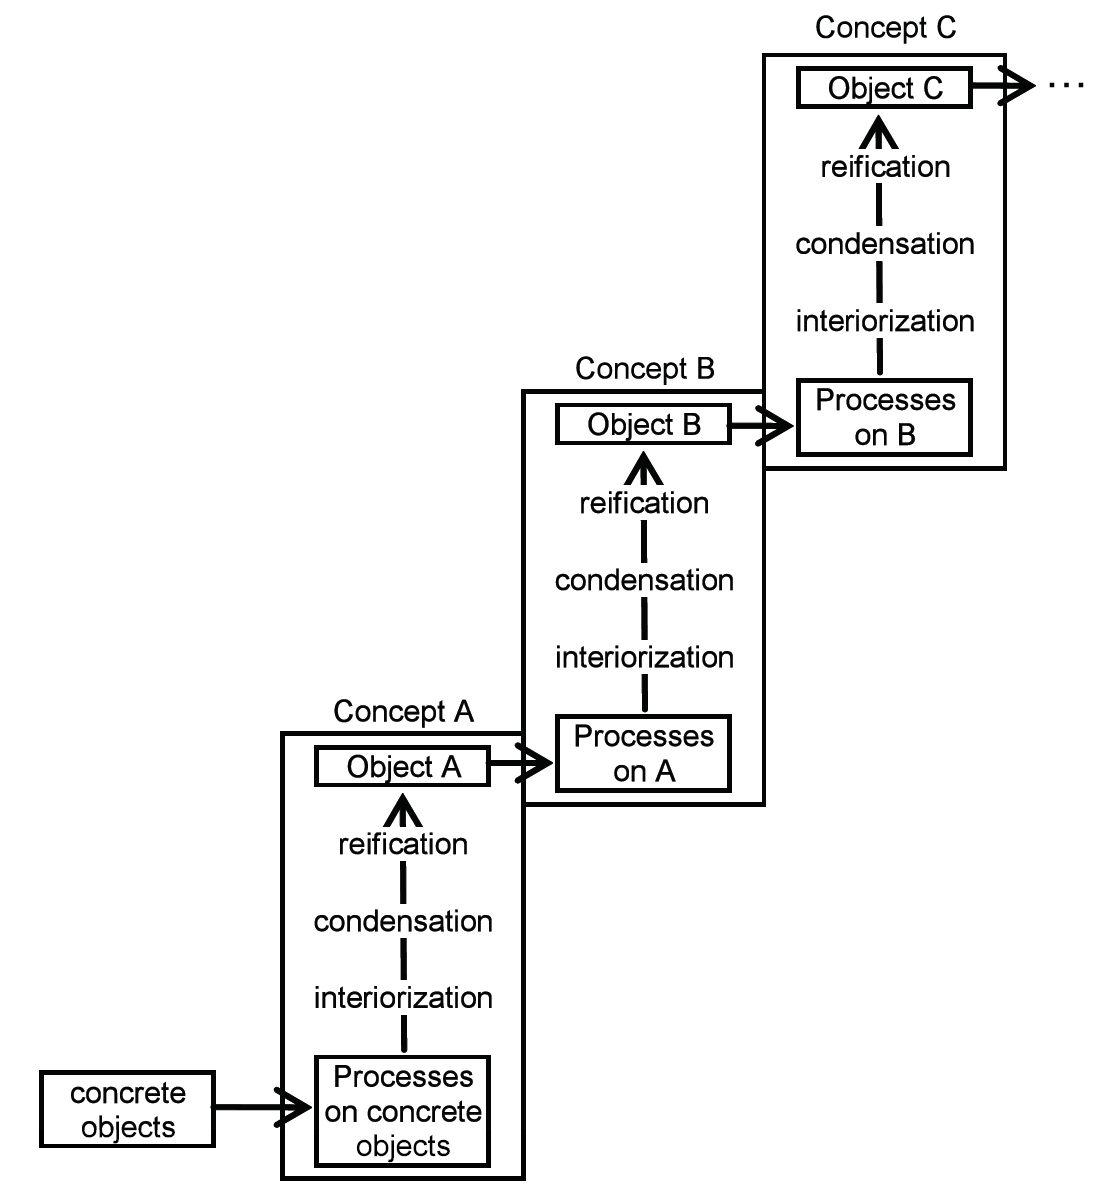
\includegraphics[scale=0.8]{figures/ListerFases.png}\label{fig:ListerFases}
%\caption{General model of concept formation (2010Lister), after Sfard (1991)}

\begin{figure*}
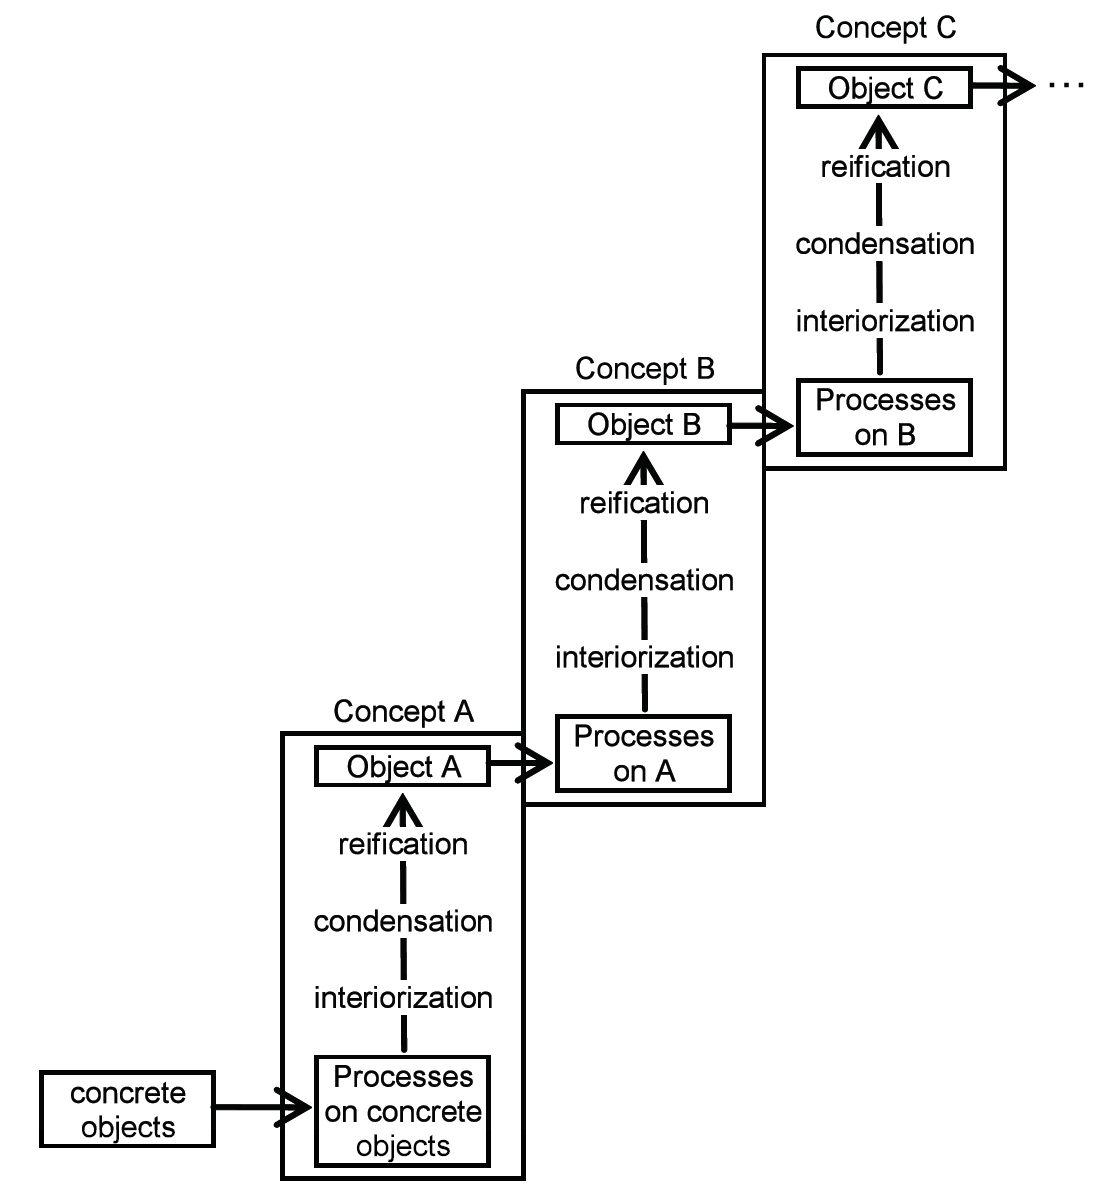
\includegraphics[scale=0.8]{figures/ListerFases.png}
\caption{General model of concept formation (2010Lister), after Sfard (1991)}\label{fig:ListerFases}
\end{figure*}


Similar to \citeA{lister2004multi}'s viewpoint on describing attainment levels per programming concept, we believe that CT skills follow a similar model. A student who is well able of decomposing a problem may have not yet evolved skills in applying generalization. Assessments should enable the identification of a student's level of competency for each particular CT skill individually.


\citeA{denning2017remaining} calls for competency tests which are supported by guidelines for different skill levels of CT. Similar to the neo-Piagetian stages (pre-operational, concrete operations, and formal operational) \cite{szabo2014neo}, he uses Dreyfus' model of progression from beginner, advanced beginner, competent, proficient, expert, through to master.

CAS has made a start (work in progress) on establishing Computing Progression Pathways and rubrics \cite{Dorling2014CTprogressions} to identify the major knowledge areas (concepts) and related CT skills of computing. It provides specific indicators of increasing levels of mastery (e.g. distinguishing between ‘understands’ and ‘can apply’) of the subject in those areas \cite{Giordano2015}. However, the framework does not discuss abilities to be acquired \cite{denning2017remaining} (see section \ref{sec:CTdef} for a discussion about abilities and skills).\todo{hebben ze ook rubrics gemaakt?}






\todo{ Erik: Licht toe en zet tegen elkaar af: “de ene onderzoek maakt wel onderscheid tussen verschillende… maar niet…”} \todo{ Nesten is een complexiteit op zichzelf
“Afhankelijkheid is geen onderdeel van de onderzoek van… “}





\subsection{Assessment practices}
This section will discuss how assessments are currently practiced in other countries and some best practices for determining levels of mastery. Curricula similar to the new Dutch curriculum are considered only.



AP CS Principles: summative written exam (2 hours, counts for 60\% of total score \& Create Performance Task (12 hours, counts for 24\% of score \& Explore Performance Task (8 hours, counts for 16\% of score).

Notes:
\begin{itemize}
\item The written exam consists of (single and multiple-select) MC questions and evaluates CS conceptual knowledge and Computational Thinking practices.
\item The Create Performance Task requires students to iteratively develop a program (using concepts such as expressions, operators, selection, iteration and/or collections) on a topic of choice. Deliverables include source code, a written report, and a 1-minute video demonstrating the program running. In the written response, the student must describe:
     \begin{itemize}
     \item The purpose of the program.
     \item The incremental and iterative development process, including difficulties and/or opportunities encountered and how they were resolved or incorporated.
     \item An independently developed \emph{algorithm} (which integrates two or more algorithms and mathematical and/or logical concepts) and how the program code segments help the program run and achieve the intended purpose of the program.
     \item An individually developed \emph{abstraction} (which integrates mathematical and logical concepts) (i.e. procedures, parameters, lists, abstract data types, APIs, libraries) and how this helps manages the complexity of the program.
     \end{itemize}
     Note that the written response includes CT aspects of algorithmic thinking, abstraction and evaluation.
\item The Explore Performance Task is not relevant for this research.
\end{itemize}
The College Board has published rubrics and annotated and marked exemplar work on their website.

\subsubsection{Programming assessment practices}\label{sec:progAssessPractices}

\todo{Inleiding: Assessing Algorithms through programming}
In this section we describe current assessment practices based on programming tasks. Programming assessments are typically used to assess both programming knowledge as programming skills. Inexplicitly and only partially, this may also include the assessment of algorithmic concepts and CT skills.


This can take different forms, from individual written exams to programming group projects. In this section we describe different types of tasks used in practice to assess programming knowledge and skills.


%types of tasks; what evidence is elicited and how
%types of knowledge being assessed (refer to taxonomies)
%anything we know about results?
% ECS and AP CS principles is validated
% what parts of assessment are standardized and validated, what do independent teachers do themselves?
% how does quality assurance take place? (i.e. New-Zealand (of AUSTRALIA??) via transparent online per-review in which all feedback and refinements are shown openly, CAS sharing via online medium in which feedback/refinements is optional (likes??) )??


\subsubsection{Algorithms assessment practices}
\todo{inleiden}
Traditionally, assessment of algorithms takes place through programming: reading or writing code. Section \ref{sec:progAssessPractices} gave an overview of programming assessment practices, here we discuss other additional approaches which specifically assess algorithms.

%verwijs naar CS principles die pseudocode gebruikt
% verwijs naar ECS die woorden en situaties gebruikt
% verwijs naar Bebras die in woorden puzzeltjes gebruikt
% zie ook vragen bij programming assessment practices


Algorithms, algorithmic thinking, and the efficiency of algorithms have been positioned at the core of a new CS curriculum being implemented in Israeli high schools\cite{gal2002efficiency}. \cite{gal2002efficiency}'s research concludes that this is a difficult concept for students.


\subsubsection{CT assessment practices}
\todo{inleiden... gaat dit hieronder niet over onderzoek ipv practices..  Er wordt toch alleen CS principles, ECS echt via practices getoetst? Ook Israel (see grover 2017assessment)??, en New zealand ook deels (is dat expliciet??). Hier juist die laatste dingen benoemen!}

In this section we discuss the ways in which, currently, some curricula assess CT.

To identify learning goals and provide student feedback on programming lab assignments, \citeA{catete2017framework} established and tested learning-based rubrics for computational thinking for AP CS Principles programming lab assignments. She concludes that teachers are able to the rubrics to achieve consistent ratings of evidence of computational thinking in student code.

\noindent\textbf{Israel national curriculum}
2013Zur-Burgury et al.\todo{cite}, describe and evaluate Israel's 2012 CS nationwide middle-school exam. The curriculum is based on the idea that CT is the key for understanding CS, and its exam specifically evaluates students' ability to deal with algorithmic thinking. The exam comprised of 9 multiple choice and open-ended questions. The questions focus on simple conditional and loop structures. Students were asked to trace, debug, complete, analyze, reason about, and compare two different programs.

\noindent\textbf{AP CS Principles}
AP CS Principles\todo{cite naar AP CS PRINCPLES GUIDE BOOK} defines 6 Computational Thinking practices: P1. Connecting computing, P2. Creating computational artifacts, P3. Abstracting, P4. Analyzing problems and artifacts, P5. Communicating, and P6. Collaborating. These practices are assessed in multiple manners. All aspects are assessed\todo{komen aan bod} in the MC written exam. In addition, all 6 return in the through-course performance tasks.

\noindent\textbf{ECS}
The ECS \todo{cite naar ECS TEACHERS BOOK} curriculum comprises of six units. Problem-solving skills and computational practices are emphasized throughout the course. Each unit has kinesthetic activities and daily collaborative and context-rich assignments to help scaffold their knowledge. Each unit has a final unit project which provides the student with an opportunity to expand and show their understandings to a particular problem. SRI has developed validated unit assessments for each of the first four units (1. Human computer interaction, 2. Problem solving, 3. Web design, and 4. Introduction to programming) as well as a cumulative assessment. Teachers are encouraged to determine which activities might make useful assessments.


\noindent\textbf{IB}



\subsection{(Design?) Methods}
This section will discuss methods used to design assessments, such as alignment methods and ECD.

\todo{Lye en Koh toetsen alleen concepten, Zhong zegt dat je alle drie aspecten moet pakken. Hoe krijg je dat nou voor elkaar?}

The Dutch curriculum description includes high-level goals \cite{Barendsen2016}. This description is not specific enough for creating assessment tasks. For example, it lacks a description of the required cognitive levels and the characteristics with which a student could show, or a teacher could determine achievement. A general approach of designing aligned assessment is to articulate an assessment argument with concrete learning outcomes and specified level of comprehension (according to a particular taxonomy)\cite{biggs1996}. Regarding the situation with the UK national curriculum, we see similarities with the Dutch. The UK levels\todo{Erik: Standards?} from the previous ICT curriculum have been removed, leaving assessment at KS3 to the responsibility of individual schools. CAS members (in co-operation with CAS Master teachers, teachers and academics) have taken the initiative to establish computing progression pathways and rubrics to assess learners' Problem-solving and Computational Thinking capabilities (Dorling and Walker, 2014).\todo{Erik: ook iets over australian standards?}\todo{Iets over NZ standards?}


In New Zealand, "progress outcomes" for CT progressions have been formulted for the Digital Technologies and mapped to the current NCEA achievement standards. These computational thinking progressions are described in terms of CS conceptual knowledge and skills: "Algorithms", "Programming", and "Data representation". At NCEA level (thus higher secondary education), its description relates to CT skills such as decomposition, algorithmic thinking, evaluation. The progression shows an uneven spacing of the progress outcomes, reflecting the different learning and time required for each outcome and is based on data collected during the development of the digital learning progressions.\todo{cite to: 2018 NZ DT curriculum development paper}

\todo{AUSTRALIA CHECK OUT}
%Australian Curriculum, Assessment and Reporting Authority. (2015). Digital Technologies: Sequence of content F-10. Retrieved from http://docs.acara.edu.au/resources/Digital_Technologies__Sequence_of_content.pdf
%
%
%Australian Curriculum, Assessment and Reporting Authority. (n.d.). Technologies: Sequence of achievement. Retrieved from http://docs.acara.edu.au/resources/Technologies_Sequence_of_achievement.pdf


Their work is based on the CT definition from the CSTA five dispositions/attitudes and builds on the work of \citeA{BrennanResnick2012}. With it, learning objectives and potential evidence observations have been established for both CS concepts and CT skills. There is no specific evidence of a structured alignment-process in the creation of assessment tasks. Importantly, \citeA{Giordano2015} concludes that designing questions which are clearly linked to the competencies is perceived as the most difficult task in the assessment process. Moreover, the more authentic and realistic, the more complex the detailed mapping to the abilities/competenties becomes. This is very relevant, as the curriculum committee follow a concept-context approach \cite{Barendsen2016}. This authentic learning approach encourages students to connect real world problems to the subject matter at hand, increasing meaningfulness and relevance. In their paper, \citeA{goode2014curriculum} emphasize why this makes sense: "engaging students in the context of complex, meaningful projects that require sustained engagement, critical thinking, collaboration, management, communication, and management of resources to develop final products or presentations builds the types of 21st century skills advocated by new sets of national standards". Especially when dealing with more complex tasks, to ensure a valid assessment, explicit alignment between learning objectives, specifications of which evidence infers the attainment of an objective, and tasks to evoke this evidence seems promising.


Based on his observations on teachers collaborating on assessment tasks, \citeauthor{hermansen2014reworking} suggests that teachers should transform (rather than implement) assessment tasks. Development and refinement yields assessments adapted to specific local settings, adhering to the needs, knowledge, skills and interests of their own students. Customizing assessment to specific local settings is a key issue. Firstly, it supports pedagogical link-making described by \citeA{scott2011pedagogical} as being fundamental to science learning. Secondly, it fits in seamlessly with an authentic concept-context approach where the assessment is to be modified according to the chosen context. Thirdly, it has the potential to promote inclusion. All-in-all, enabling teachers to create tasks which are fine-tuned to their specific classroom needs may well be a fruitful method to establish qualitative assessments.
%bare necessity for implementing a concept-context approach.


%\subsubsection*{Learning objectives and KSAs}
\todo{ Naar achtergrond met meer toelichting, uitleggen. What is abilities (niet attitutes?)? What is verschil tussen skill en abilities?}
\todo{Why needed}


\note{knowledge, skills or other attributes}
%
%linked to evidence-eliciting-performances



\subsubsection{Evidence-Centered Design}\label{sec:ECD}
Initiatives in the U.S. follow a structured path, incorporating validity evidence into an assessment design process. SRI International, an independent, nonprofit research center serving the U.S. government, launched a Teacher Assessment Literacy for Exploring Computer Science study to investigate the design and delivery of high-quality assessment materials. They apply the Evidence-Centered Design (ECD) method. ECD is a principled method for modeling domains for assessment purposes that is especially useful for hard-to-assess practices \cite{grover2016assessing}. Table \ref{fig:ECD} gives an overview of the processes and products of each of the five ECD layers. ECD's systematic structure facilitates a coherent mapping from high-level curricular goals to observable behaviors. This yields three models designed to elicit evidence of students' achievement levels of the relevant learning objectives.
\begin{itemize}
\item The \emph{student model} specifies the knowledge, skills or other attributes (KSA) to be assessed.
\item The \emph{evidence model} describes observable behaviors or performances which may provide evidence about the KSAs, and thus links the chain of reasoning from students’ performances to their knowledge and skills.
    \note{Evidence models lay out the argument about why and how observations in a given task situation constitute evidence about student model variables. There are two parts to an evidence model, the evaluation component and the measurement component.}
\item The \emph{task model} describes the environment in which students say, do, or make something to provide evidence.
\end{itemize}

Evidence is obtained by deliberately putting students in those situations, with challenges, or tasks that will elicit the desired KSAs (Grover and Bienkowski, forthcoming). \citeA{mislevy2006implications} report on the application of this method has received many citations. This methodology was recently applied in CS by \citeA{grover2017measuring} to assess problem-solving processes, and for the development of assessment instruments for the Exploring Computer Science curriculum by \citeA{McGee2018ECS}, \citeA{rutstein2014computational}, and \citeA{snow2017CTECD}). ECS incorporates both CS concepts and CT skills.





\begin*{table}
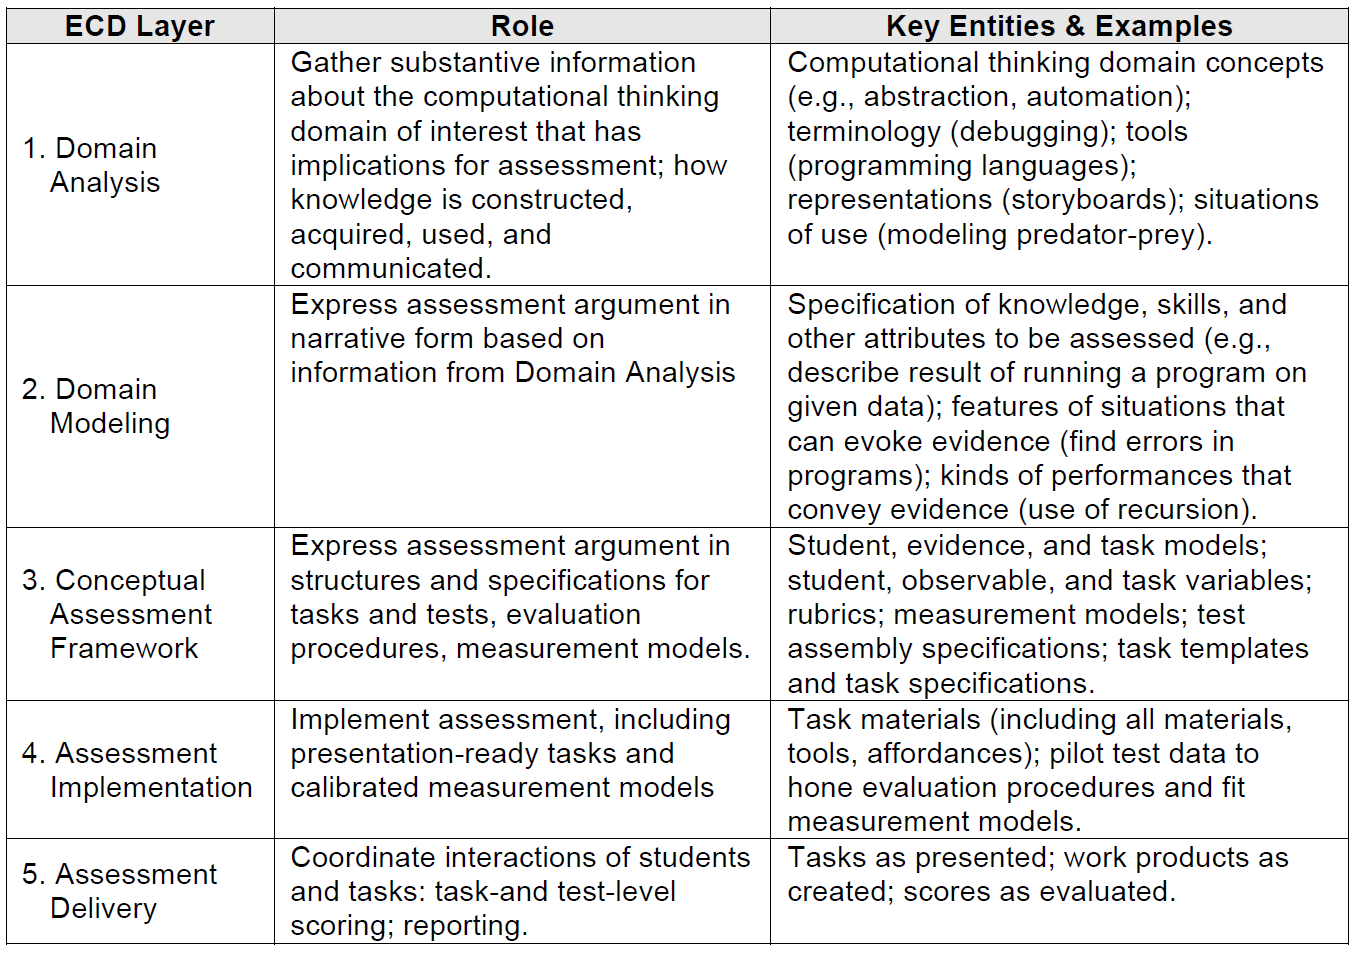
\includegraphics[scale=0.8]{figures/ECDoverview.png}
Roles and Key Entities in the Five Layers of Evidence-Centered Design (\todo{cite}2014SnowBienkowski)\label{fig:ECD}
\end*{table}





%\begin{itemize}
%\item \textbf{Domain Analysis:}
%The top layer in the ECD process is a Domain Analysis to clarify learning goals.
%This level includes determining relevant concepts and terminology,(e.g. abstraction, algorithms), tools (i.e. programming languages) and representations (flowcharts, pseudocode) as well as understanding how knowledge is constructed, acquired, used and communicated (SRI Assessment Design Patterns for CT, 2017). In the process, the curricular learning objectives are translated into more specific and learning goals specified in operational terms, ready for teacher use
%\item \textbf{Domain Modelling:} the assessment argument was designed. The learning goals were translated into the specific focal knowledge, skills, and attributes (KSAs)
%
%\item \textbf{Conceptual Assessment Framework:}
%The result of this phase was a design pattern consisting of three aligned models (student model, evidence model, and task model) which together form the assessment specifications: the foundation for the new assessment.
%
%\item \textbf{Assessment Implementation:}During the implementation stage, the model assessment tasks are translated into classroom-specific assessment tasks in the designated programming language.
%
%\item \textbf{Assessment Delivery:} the tasks are administered to students.
%\end{itemize}



%This methodology has been used by, extensively reported on, and cited to by Mislevy et al. (2002, 2003).



\subsubsection{Expert panel}\label{sec:ExpertPanel}
While establishing assessments, transitioning from one layer of abstraction (i.e. high-level curricular goals) to the next (KSAs) involves analytical precision and careful reasoning. In this section we describe methods for several experts to review the process's results and come to a consensus\todo{meningsverschillen plat te strijken.}.


Several methods can be used to resolve differences in opinions and obtain an objective consensus between panel members, such as focus groups\todo{ref WIPSCE artikel over thresholds}, Nominal Group Technique\todo{Adler, M. and Ziglio, E. Gazing into the oracle: The Delphi method and its application to social policy and public health. Jessica Kingsley Publishers, 1996.} or the Delphi method\todo{ref brooks 779}.

The purpose of the Delphi technique is to test opinion consensus amongst a group of experts. It is usually employed in research where there is a high level of uncertainty or the collective opinion of experts would be beneficial \cite{kallia2017assessment}. Using this technique, a group of experts is brought together (either virtually or physically) to answer a question. After the first round, the participants' responses are shared anonymously, and the question is re-stated. This process repeats until a consensus is reached. In his study on consensus methods, Vernon (2009)\todo{cite} states that consensus values generally lie between 55\% and 100\%, with a modus of 70\%.




CS Principles (CSP) was first designed for the college level and then used as a basis for secondary education AP CS Principles. However, the standards were established for expert programmers and not described in enough detail to assess beginner-level skills. To help teachers identify learning goals and provide student feedback on programming lab assignments, \citeA{catete2017framework} established and tested learning-based rubrics for computational thinking. She systematically determined quality criteria and then made use of expert panel (a combination of the Delphi method and Nominal Group Technique) for validation purposes.

\todo{  DELPHI?? De moeite waard? Misschien delen van DELPHI methode gebruiken? Kijk evt naar artikel over thresholds WIPSCE, evt met een focusgroep (is sneller en minder zwaar aangezet). Beschrijf hier hoe je verschillen gaat oplossen. Relateer evt ook aan ECS ECD met DELPHI. Elementen van methode gebruiken, niet hele methode, Nominal Group Technique? (zie 2017 catete.}

\todo{Kallia, Sentance WIpsce 2017 Computing Teachers' Perspectives on Threshold Concepts describe and use the delphi method}




\subsubsection{Research assessment methods and tasks}
We now discuss researches pertaining to assessment tasks.
%, including the fit-for-use and fit-for-purpose criteria.\todo{Criteria according to the wheel of assessment?}


Gathering evidence of task performance can take many forms:
\begin{itemize}
\item written exams
\item short programming assignments, such as used in Informatics Olympiads \cite{Lonati2017Bebras}
\item (open-ended) projects (and the end of, or across an entire course)
\item charettes (fixed-length laboratory assignments)\todo{cite}
\item game design tasks \cite{snow2017CTECD}
\item (CT) puzzles, such as used in Bebras competition (Dagiene and Sentance, 2016)

\end{itemize}


The deliverables of a project can be:
\begin{itemize}
\item written report,
\item digital artifact,
\item comments in code,
\item presentation,
\item logbook,
\item self-reflection,
\item project notes,
\item creative design report
\end{itemize}
or a combination of one or more of these.


Depending on the task performance chosen, methods to determine levels of mastery can be:
\begin{itemize}
\item analysis of deliverable mentioned above \todo{what to look for, such as in a reflection report}

\item specifically, analysis of digital artifacts  \cite{BrennanResnick2012} \todo{what did they look for}, and constructs used \todo{Dr. Scratch}

\item artifact-based interviews (Grover et al., 2015)
\item real-time observations
\item \ldots
\end{itemize}


Written exams themselves can have tasks of different nature. \citeA{lister2010naturally} summarize a few:
\begin{itemize}
\item \emph{multiple-choice questions}: Multiple-choice questions are closed and are primarily used to assess at a unistructural level \cite{Zhong2016} and at a low cognitive level on Bloom's taxonomy, namely Remembering and Understanding\cite{zur-burgury2013israelExam}. According to \citeA{2010TewGuzdial} when constructed carefully, multiple-choice questions can provide the same information about conceptual knowledge as short answer or open response questions with significant advantages in test administration and scoring. \cite{zur-burgury2013israelExam} state that by constructing questions appropriately, the Evaluating and Creating cognitive levels can be assessed. For example, for a student to complete the skeleton of a script, the students need to understand the algorithmic problem, the proposed solution, and must complete the missing parts. Morrison and Free (2001) also explain that they can be used to assess higher-order thinking. Due to their clear advantages of being objective and easy to mark, many courses use multiple choice tests. However, distracters must be selected carefully.
\item \emph{multiple-choice combined with open}: Students select a multiple-choice answer and include an explanation of their response choice. Incorrect answers are graded easily. Asking students to formulate their reasoning ensures students aren't just guessing. Misconceptions are easily detected, facilitating feedback. These types of questions are used in the ECS exam, and has also been used by \cite{gal2002efficiency} to assess analyzing and efficiency of algorithms.
\item \emph{debugging questions}: the student is given code and asked to locate and correct an error.
\item \emph{tracing}: the student is asked to predict an outcome or describe (i.e. summarize)the goal of a code selection. Thompson (2016) looked at "explain in plain English" tasks and conclude that despite that they may be ambiguous, they are a reliable indicator of a student’s ability to respond relationally.

\item \emph{modifying}: the student is given code and asked to adjust it to achieve a particular goal.
\item \emph{Parsons problems}: All the required code to solve a problem is provided in random order, and students must be rearrange these into the correct order. Whilst lowering the cognitive load, Parsons problems can be used to focus assessment specifically on misconceptions or areas that learners typically struggle, and their difficulty is easily adapted \cite{ericson2017parsons}. A clear advantage is that marking is fast and objective. Students complete Parsons problems faster than writing code. \citeA{denny2008parsons} note a direct correlation between Parsons-problem and code writing scores.
\item \emph{semi-open}: Fill-in-the-blank type questions. \todo{According to the description of open and semi-open tasks used by \citeA{Zhong2016}, a mapping to multi-structural and relational cognitive levels on the SOLO taxonomy seems plausible}
\item \emph{open}: Such as, write a program to solve an algorithmic problem (used by \citeA{gal2002efficiency}).\todo{harder to mark: more time, less objective}\todo{According to the description of open and semi-open tasks used by \citeA{Zhong2016}, a mapping to multi-structural and relational cognitive levels on the SOLO taxonomy seems plausible}
\end{itemize}



Due to the both the cognitive and non-cognitive aspects of learning CT, multiple measures contribute to an accurate picture of the students capabilities. Some tasks may be better suited to elicit particular (levels) of attainment than others. In order to give students ample possibility to provide evidence of their knowledge and skills, assessments should assess on multiple cognitive levels. In their research, \citeA{grover2017measuring} argue for a multi-facetted assessment. There has been quite some research done on the effectiveness of different types of assessments, each with its own advantages and disadvantages. \citeA{BrennanResnick2012} use multiple approaches to assess student's learning.




%CS1 much research to assessment tasks: mc, parsons, sniplets,
%meet the criteria in \ref{sec:qualityCriteria} in addition
\todo{kijken waar dit hoort:}
In his review on developing generic resources for assessment, Hermansen (\cite{hermansen2014reworking}4) concludes, based on several researches, that assessment tools aren't plug-and-play modules that can be relocated and implemented as-is. Rather, in order to remain operable they must be adapted and 'recontextualized' according to classroom needs.

Concluding, many different types and forms of tasks and situations can be used to elicit evidence about a student's knowledge and skills. For a complete picture of attainment levels for both CT skills and CS concepts, a mix of assessment forms should be used.

\subsubsection{Assessment methods and tasks in practice}

\todo{Make a table with different curricula and their exams: AP, ECS, NEW ZEALAND, ISREAL}
\todo{koppelen aan criteria in \ref{sec:qualityCriteria} }
\todo{verschillende soorten vragen/opdrachten}

And indeed, MC-questions appear in AP CS Principle exams to assess computational thinking skills (in line with Morrison and Free (2001) and 2010TewGuzdial)

\todo{Israel,SEE:
I. Zur Bargury, 2012. A new Curriculum for Junior-High in Computer Science, ITiCSE'12, Haifa, Israel,  p. 204-208, ACM.
I. Zur Bargury et al., 2012. Implementing a New Computer Science Curriculum for Middle School in Israel, FIE’12, Seattle, Washington, p.886-891}

\subsection{PCK (THEORY)}
Effective teaching requires a combination of pedagogy, content, and knowledge (PCK) \cite{shulman1986pedagogical}. In a nutshell, PCK means that subject matter (content knowledge) and ways of teaching (pedagogical knowledge) are integrated \cite{Yadav2016}. It encompasses knowing what makes certain topics easy or difficult, as well as ways of representing and formulating topics in different ways \cite{shulman1986pedagogical}. This section will describe PCK of computer science teachers pertaining to the concepts in this research. In this research we focus on one of the four aspects of PCK, namely assessment. We are particularly interested in the PCK aspects needed to adapt and implement particular types of assessment, those that elicit knowledge and skills pertaining to algorithms and algorithmic thinking.\todo{Erik: PCK is niet een geheel ding, maar topic specifiek}

Magnusson, Krajcik en Borko (1999) distinguish four aspects of content-specific PCK: knowledge of
(1) curricula, (2) students' understanding and difficulties, (3) instructional strategies, and (4) assessment.

In their paper, \citeA{Kao2018} propose and piloted a 9 question pre-test and post-test to assess different aspects of CS PCK amongst pre-AP and AP CS teachers. They specified several important CS PCK characteristics, particularly teachers' knowledge of explanations, suboptimal solutions, and misconceptions.  In their PCK based research, \citeA{Yadav2016} interviewed high school teachers in the U.S. to understand the challenges they face. The challenges they found include isolation, lack of adequate computer science background, and limited professional development resources.

\citeA{yadav2014computational} piloted a module to teach CT to pre-service teachers and concluded that it was effective in influencing teacher's understanding and positive attitude toward CT and its integration into the classroom. Thus, Teaching PCK explicitly seems to be effective.

\todo{Erik: verwijzen naar Natasa}
\todo{Erik: lezen over en verwijzen naar m. saeli over pck programmeren, samen iets met Bert Zwanneveld en Jochems geschreven}


\todo{A strong PCK of these 3 aspects interconnection is an indicator for quality of teacher's PCK, strong conncetions contribute to strong PCK}

%\todo{benadrukken dat het content/onderwerp specifiek is.. dus CT PCK kan voor een bepaald docent op een heel ander ontwikkelingsniveau zitten dan Programmeren PCK}



From his extensive literature review, Hermansen summarizes that teachers who implement formative assessment resources "draw upon a strong understanding of subject knowledge, use a range of ideas and tools to enable classroom interaction and learning, have established a new division of labour in their classrooms, focus on developing student learning and autonomy, and critically examine their own beliefs about learning and classroom practices". This list alone affirms that any teacher new to teaching, or new to a particular concept, will likely be lacking some, if not all of these skills or knowledge.


\todo{kijken waar dit hoort:}
Because assessment, let alone multi-facetted assessment, can be a daunting tasks, teachers should work together or use template assessment tasks which they can adapt to their own specific classroom needs.



\subsubsection*{Assessment (as an aspect of PCK) in practice}
This section will describe PCK of computer science teachers in practice.
\todo{deze hoofdstuk nog even goed doorlezen en aan elkaar praten}

Very little is known about PCK for Computing \cite{Yadav2016}. As an aspect of PCK, teachers have limited knowledge about assessment and seriously struggle with it \cite{popham2009assessment}. Particularly, teachers face many challenges with respect to the assessment of new topics (DeLuca and Klinger, 2010). The 2015 study by Computer Science Teacher's Association (CSTA) found that teachers have trouble finding valid and reliable assessments to use in their classrooms. Along the same line, Dutch teachers say they lack qualitative (peer-)reviewed materials, assessment rubrics and access to question banks \cite{tolboom2014informatica}.


\citeA{Oliver2004} found that CS teachers assess merely a small spectrum of levels in Bloom's taxonomy. This was confirmed by \citeA{Whalley2006}. Depending on the particular concept, in some cases only the lower knowledge levels are assessed (networks), in others predominantly the higher application and analysis levels (programming). Either way, this leads to non-discriminative assessments.


Even if there is published material available, many teachers create and rely on their own material \cite{popham2009assessment}.

Faced with a specific assessment task, teachers generally take previously developed templates as a point of departure and adapt them to meet their current requirements \cite{hermansen2014reworking}. During his observations he saw that teachers spent significant time on aspects pertaining to the elicitation of evidence of students' capabilities. This indicates that teachers are well-informed about the role of an assessment. \citeA{Yadav2015} conclude that teachers lack PCK, which manifests itself in an incapacity to act: the teachers understand need for qualitative assessment, but just don't know how to.

%Both experienced and novice teachers struggle in assessing student learning (Fincher, Kolling, Utting, %Brown, Stevens 2010)(Hebert \& Worthy, 2001)(Veenman, 1984) (Yadav, 2016)(Yadav, %2015)(Bardensen et al., 2015 ITICSE wg).


Thus, judgements about students' proficiency are made without the use of validated, sometimes not even valid assessments. \citeA{Whalley2006} describe the assessment of programming as complex and challenging and emphasize the lack of clear frameworks and tools. \citeA{ragonis2012type} state that if the quality of assessment is insufficient, teaching will be ineffective. \citeA{Giordano2015} add that if teachers use low-quality assessment instruments we will end-up teaching the wrong subject, and vice-versa.


Teacher educators need to provide teachers with the content, pedagogy, and instructional strategies needed to incorporate computational thinking, and in particular the assessment of the its core concepts \cite{Yadav2017CTteacherEd}.







